\newpage
\hypertarget{schema vis}{}
\subsection{Visual Schema}
\visHeader

\begin{itemize}

\item[$\blacktriangleright$] Open \texttt{LeitnersLearningBox} in EA, and add a new package to your model root, \texttt{My Working Set}. Name it
\texttt{Learning\-Box\-To\-Dictionary\-Integration} (Fig.~\ref{fig:intgPackage}).

\vspace{0.5cm}

\begin{figure}[htbp]
\begin{center}
  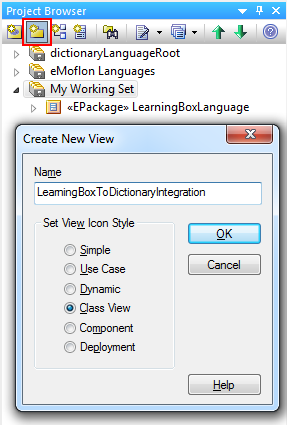
\includegraphics[width=0.5\textwidth]{ea_integrationPackage}
  \caption{Create a new package}  
  \label{fig:intgPackage}
\end{center}
\end{figure}

\item[$\blacktriangleright$] Create a diagram in the new package, selecting \texttt{TGG Schema} as diagram type (Fig.~\ref{fig:tgg_diagram_type}). The diagram
type indicates to EA that the new package is a TGG Project.

\vspace{0.5cm}

\begin{figure}[htbp]
\begin{center}
  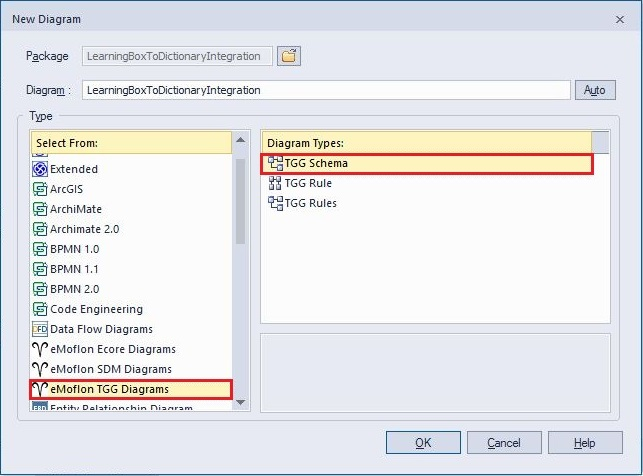
\includegraphics[width=0.9\textwidth]{ea_newTGGSchema}
  \caption{Choose \texttt{TGG Schema} as your diagram type}  
  \label{fig:tgg_diagram_type}
\end{center}
\end{figure}

\item[$\blacktriangleright$] A dialogue should pop up asking you for the source and target projects of your TGG project.  Choose
\texttt{Learning\-Box\-Language} as source and \texttt{Dictionary\-Language} as target project and affirm with \texttt{OK} (Fig.~\ref{fig:select_source_target}).

\vspace{0.5cm}

\begin{figure}[htbp]
\begin{center}
  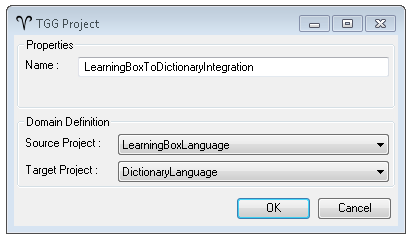
\includegraphics[width=0.55\textwidth]{ea_TGGSourceTarget}
  \caption{Select source and target projects for the TGG project}  
  \label{fig:select_source_target}
\end{center}
\end{figure}

\item[$\blacktriangleright$] The structure of your TGG project should now resemble Fig.~\ref{fig:new_tgg_project}. Please note that a subpackage \texttt{Rules}
and an underlying diagram with the same name are also generated.

\begin{figure}[htbp]
\begin{center}
  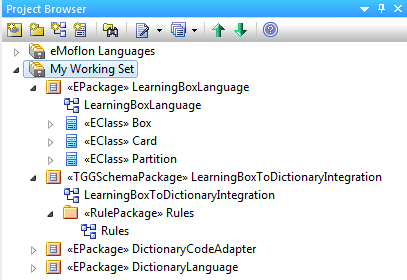
\includegraphics[width=0.5\textwidth]{ea_browserPostDiagram}
  \caption{Initial structure of a new TGG project}  
  \label{fig:new_tgg_project}
\end{center}
\end{figure}
\end{itemize}
\clearpage

Now it's time to insert classes from our source and target projects into our TGG project and declare our first \emph{correspondence type} between them.
The classes \texttt{Box} and \texttt{Dictionary} are to be related to each other. Please note that all other information in the source and target metamodels,
such as attributes, methods, and references, are shown by default in the TGG schema.

\begin{itemize}

\item[$\blacktriangleright$] Confirm the TGG schema diagram is open in the editor and hold \texttt{ctrl}, then drag-and-drop the \texttt{Box} class from
\texttt{Learning\-Box\-Language} into the window. Ensure that the class is pasted \texttt{as a simple link} into the diagram (Fig.~\ref{fig:TGGdragDrop})

\vspace{0.5cm}

\begin{figure}[htbp]
\begin{center}
  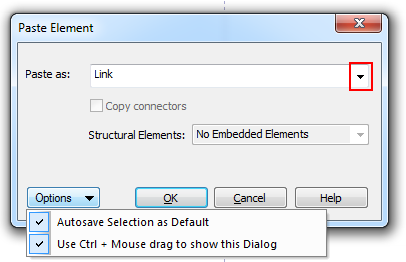
\includegraphics[width=0.6\textwidth]{ea_TGGDragDrop}
  \caption{Copying an element as a simple link} 
  \label{fig:TGGdragDrop}
\end{center}
\end{figure}

\item[$\blacktriangleright$] Note that you are able to set \texttt{Autosave Selection as default}. In fact, we did this in the previous part! We'll need to
switch drag types several times during this part however, so it's best to leave this unchecked if you do not want to hold \texttt{ctrl} each time you use the
drag-and-drop gesture.

\vspace{0.5cm}

\item[$\blacktriangleright$] With a class from both source and target metamodels, we can now create a correspondence type between them! Quick-link from
\texttt{Box} to \texttt{Dictionary}, and select \texttt{Create TGG Corres\-pon\-dence Type} (Fig.~\ref{fig:create_correspondence}).

\newpage

\begin{figure}[htbp]
\begin{center}
  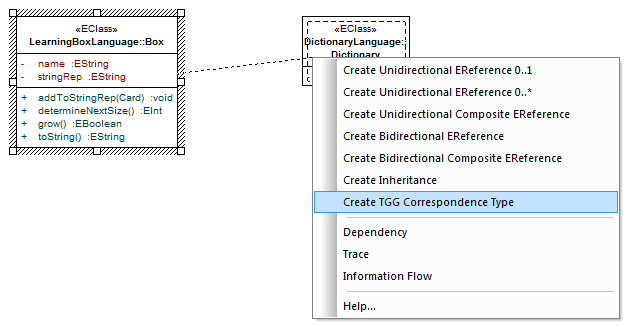
\includegraphics[width=\textwidth]{ea_TGGCorrespType}
  \caption{Creating a TGG correspondence type} 
  \label{fig:create_correspondence}
\end{center}
\end{figure}

\item[$\blacktriangleright$] As you can see, a correspondence type has been created, visualised as an hexagonal shape (Fig.~\ref{fig:ea_firstCorrType}). It is
automatically named \texttt{BoxToDiction\-ary}, and the relevant references have been generated.

\vspace{0.5cm}

\begin{figure}[htbp]
\begin{center}
  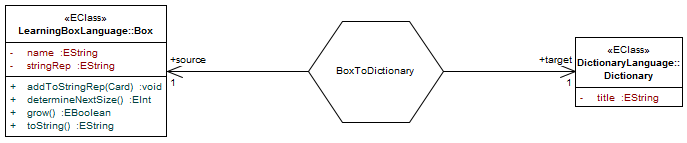
\includegraphics[width=\textwidth]{ea_firstTGGSchema}
  \caption{Creating a TGG correspondence type} 
  \label{fig:ea_firstCorrType}
\end{center}
\end{figure}

\item[$\blacktriangleright$] You're done! To see how the source and target classes, along with the correspondence type between them are declared in the textual
schema, check out Fig.~\ref{fig:firstCorrType} in the next section.

% Can this be omitted? Users create a new one on the fly?
% \item[$\blacktriangleright$] To finish our TGG schema, declare a second correspondence type in the same file between \texttt{Card} and \texttt{Entry}. You'll
% notice that the reference between \texttt{Dictionary} and \texttt{Entry} was automatically created! Your completed TGG Schema should resemble
% Fig.~\ref{fig:complete_tgg_schema}.

% \begin{figure}[htbp]
% \begin{center}
%   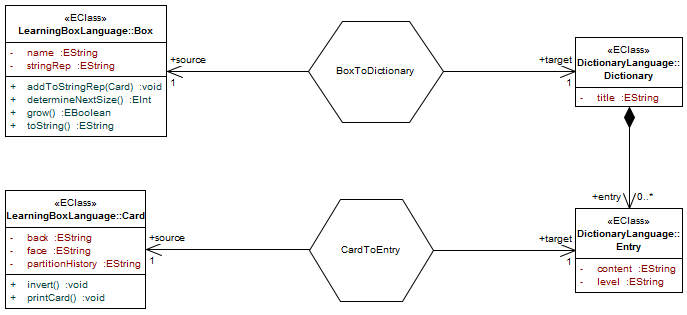
\includegraphics[width=\textwidth]{ea_completeTGGSchema}
%   \caption{Complete TGG schema for our example}
%   \label{fig:complete_tgg_schema}
% \end{center}
% \end{figure}

\end{itemize}

